\documentclass[urlcolor=blue,dvipsnames]{beamer}

\usepackage[utf8]{inputenc}
\usepackage{fancybox,fancyvrb}
\usepackage{environ,xspace,empheq}

\usepackage{tikz}
\usetikzlibrary{arrows.meta,decorations.markings,decorations.pathreplacing,fadings,positioning}

\hypersetup{colorlinks,linkcolor=,urlcolor=cyan}

\beamertemplatenavigationsymbolsempty
\setbeamertemplate{footline}[frame number]
\usetheme{Pittsburgh}

%\makeatletter
%\newcommand{\tinytiny}{\@setfontsize{\tinytiny}{4pt}{4pt}}
%\makeatother

\newcommand\enumnum[1]{{\renewcommand{\insertenumlabel}{#1}%
      \usebeamertemplate{enumerate item} \,}}

\newcommand{\grad}{\nabla}
\newcommand{\ih}{\boldsymbol{\hat{\textbf{\i}}}}
\newcommand{\jh}{\boldsymbol{\hat{\textbf{\j}}}}
\newcommand{\vF}{\boldsymbol{\vec{\textbf{F}}}}
\newcommand{\Matlab}{\textsc{Matlab}\xspace}
\newcommand{\Octave}{\textsc{Octave}\xspace}


\title{7.3 Laplace Transforms: \\ translations \& unit step functions}

\subtitle{a lesson for MATH F302 Differential Equations}

\author{Ed Bueler, Dept.~of Mathematics and Statistics, UAF}

\date{\tiny \today}


\begin{document}
\setbeamertemplate{itemize item}{$\bullet$}
\setbeamertemplate{itemize subitem}{$\circ$}
\renewcommand{\thefootnote}{{\color{green} \arabic{footnote}}}

\begin{frame}
\titlepage

\centerline{\tiny for textbook: \, D. Zill, \emph{A First Course in Differential Equations with Modeling Applications}, 11th ed.}
%\color{green!40!blue}
\end{frame}

\newcommand{\LL}[1]{\mathcal{L}\left\{#1\right\}}
\newcommand{\LLi}[1]{\mathcal{L}^{-1}\left\{#1\right\}}


\begin{frame}{the Laplace transform strategy}

\begin{center}
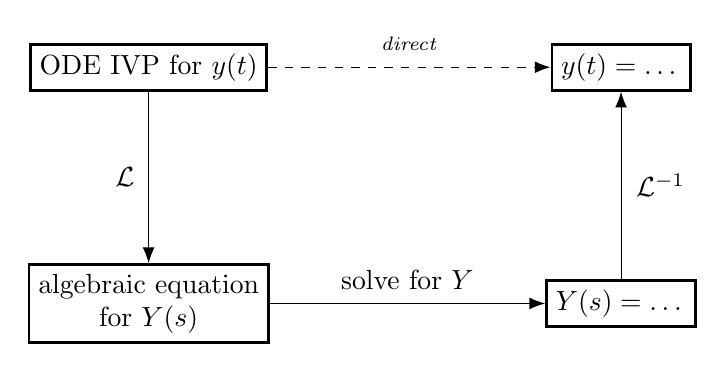
\begin{tikzpicture}[scale=1.0,>={Latex[length=2mm]},
  component/.style={rectangle,draw,fill=white,align=center,line width=1pt}]

\draw (-3,3) node[component] (ode) {ODE IVP for $y(t)$};
\draw (-3,0) node[component] (Leqn) {algebraic equation \\ for $Y(s)$};
\draw (3,0) node[component] (Lsoln)   {$Y(s)=\dots$};
\draw (3,3) node[component] (odesoln)   {$y(t)=\dots$};
\path
   (ode) edge[->] node[xshift=-3mm] {$\mathcal{L}$} (Leqn)
   (Leqn) edge[->] node[yshift=3mm] {solve for $Y$} (Lsoln)
   (Lsoln) edge[->] node[xshift=+5mm] {$\mathcal{L}^{-1}$} (odesoln)
   (ode) edge[dashed,->] node[yshift=3mm] {\scriptsize \emph{direct}} (odesoln);

\end{tikzpicture}
\end{center}

\begin{itemize}
\item \S 7.3: ``operational properties'' regarding translations (shifts)
    \begin{itemize}
    \item including the \emph{unit step function} $\mathcal{U}(t)$
    \end{itemize}
\item \S 7.4 (next): ``operational property'' re \emph{convolution}
\end{itemize}
\end{frame}


\begin{frame}{recall Laplace's Transform}

\begin{columns}
\begin{column}{0.77\textwidth}
\begin{itemize}
\item the definition:
    $$\LL{f(t)} = \int_0^\infty e^{-st} f(t)\,dt$$
\item when applying $\mathcal{L}$ to an ODE use:
\begin{align*}
\LL{y'(t)} &= s Y(s) - y(0) \\
\LL{y''(t)} &= s^2 Y(s) - s y(0) - y'(0)
\end{align*}
\item doing $\mathcal{L}^{-1}$ is mostly use of a table, e.g.:
    \begin{itemize}
    \item $\displaystyle \LLi{\frac{1}{s-4}} = e^{4t}$
    \item $\displaystyle \LLi{\frac{k}{(s-a)^2+k^2}} = e^{at} \sin{kt}$
    \end{itemize}
\end{itemize}
\end{column}
\begin{column}{0.23\textwidth}
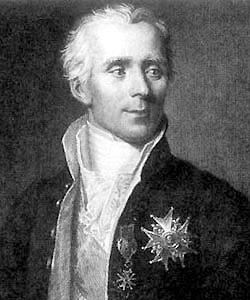
\includegraphics[width=\textwidth]{figs/Laplace-sharp}

\vspace{3mm}
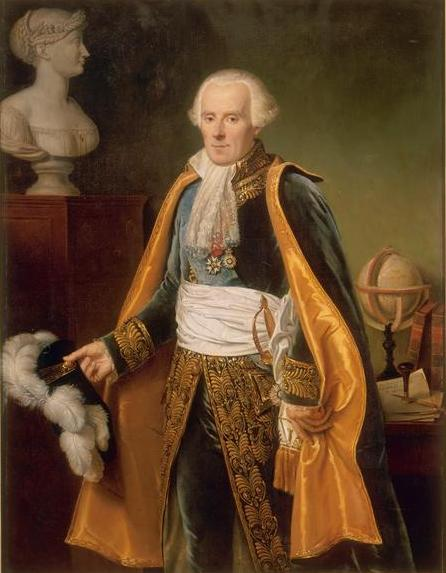
\includegraphics[width=\textwidth]{figs/Laplace-grand}

\tiny
Pierre-Simon Laplace (1749--1827) 
\end{column}
\end{columns}
\end{frame}


\begin{frame}{we have a decent table}

\vspace{-2mm}
\begin{center}
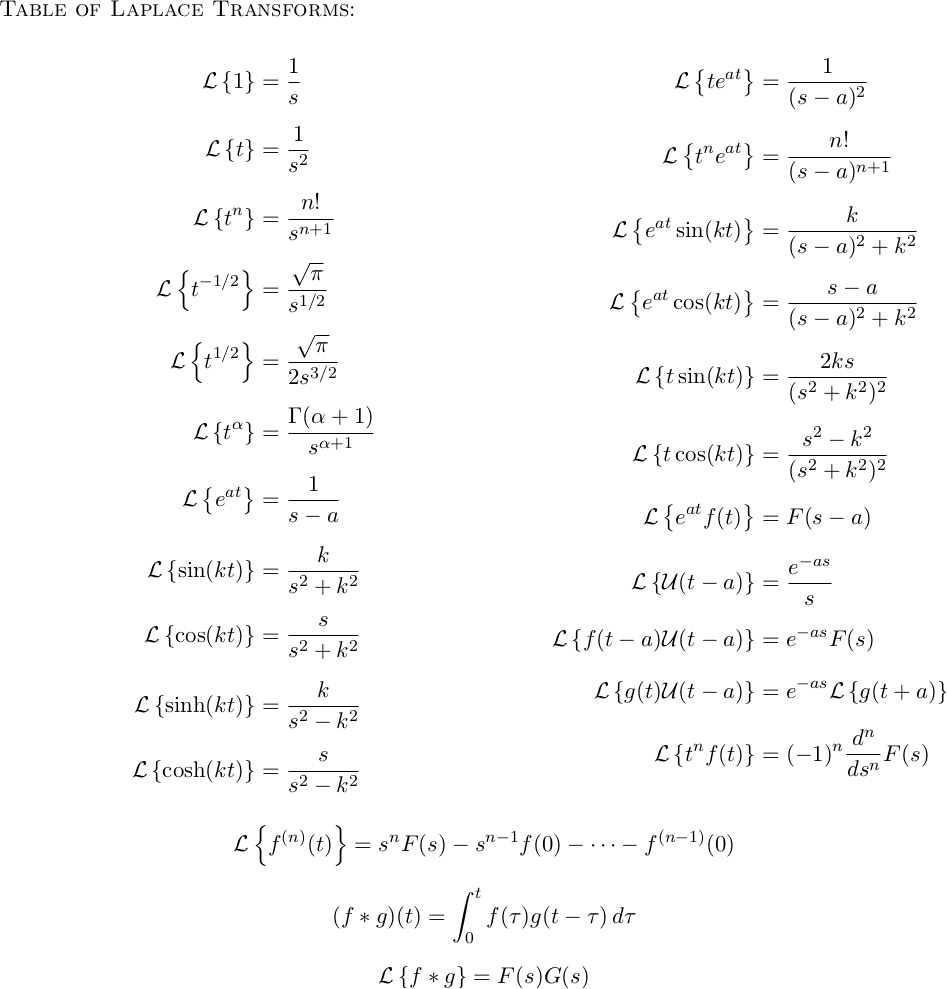
\includegraphics[height=80mm]{figs/fulllaplacetable}
\end{center}
\end{frame}


\begin{frame}{noticable in the table}

\begin{itemize}
\item compare the left and right columns in this part of the table:
\small
\begin{align*}
\LL{t} &= \frac{1}{s^2}            &&& \LL{te^{at}} &= \frac{1}{(s-a)^2} \\
\LL{t^n} &= \frac{n!}{s^{n+1}}     &&& \LL{t^n e^{at}} &= \frac{n!}{(s-a)^{n+1}} \\
\LL{\sin(kt)} &= \frac{k}{s^2+k^2} &&& \LL{e^{at}\sin(kt)} &= \frac{k}{(s-a)^2+k^2} \\
\LL{\cos(kt)} &= \frac{s}{s^2+k^2} &&& \LL{e^{at}\cos(kt)} &= \frac{s-a}{(s-a)^2+k^2}
\end{align*}
\item multiplying by $e^{at}$ causes: \, $s\to s-a$
\item this is a rule!: multiplying by an exponential in $t$ is \emph{translation} in $s$:
   $$\LL{e^{at} f(t)} = F(s-a)$$
\end{itemize}
\end{frame}


\begin{frame}{why?}

\begin{itemize}
\item \emph{why} does multiplying by $e^{at}$ cause \, $s\to s-a$ \,?
\item recall definition:
   $$\LL{f(t)} = F(s) = \int_0^\infty e^{-st} f(t)\,dt$$
\item so:
\begin{align*}
\LL{e^{at} f(t)} &= \int_0^\infty e^{-st} e^{at} f(t)\,dt = \int_0^\infty e^{-(s-a)t} f(t)\,dt \\
   &= F(s-a)
\end{align*}
\end{itemize}
\end{frame}


\begin{frame}{examples from \S7.3}

\begin{itemize}
\item start by just going back and forth using the new rule
\item \emph{exercise 1.} % like #7
   $$\LL{e^{2t} \sin(3t)} = \hspace{100mm}$$

\vspace{20mm}
\item \emph{exercise 2.} % like #13
   $$\LLi{\frac{1}{s^2-6s+10}} = \hspace{100mm}$$

\vspace{20mm}
\end{itemize}
\end{frame}


\begin{frame}{example like \S7.3 \#23}

\begin{itemize}
\item \emph{exercise 3.} use $\mathcal{L}$ to solve the ODE IVP:
    $$y''+4y'+4y=0, \quad y(0)=1, \, y'(0)=1 \hspace{40mm}$$

\vspace{60mm}
\end{itemize}
\end{frame}


\begin{frame}{example like \S7.3 \#30}

\begin{itemize}
\item \emph{exercise 4.} use $\mathcal{L}$ to solve the ODE IVP:
    $$y''-2y'+5y=t, \quad y(0)=0, \, y'(0)=7 \hspace{40mm}$$

\vspace{60mm}
\end{itemize}
\end{frame}

\newcommand{\UU}{\mathcal{U}}

\begin{frame}{unit step function}

\begin{columns}
\begin{column}{0.65\textwidth}
\begin{itemize}
\item \emph{definition.}  the \emph{unit step function} is
    $$\UU(t) = \begin{cases} 0, & t < 0 \\
                             1, & t \ge 0 \end{cases}$$
\item the book defines it with a translation, and only on $[0,\infty)$
    $$\UU(t-a) = \begin{cases} 0, & 0\le t < a \\
                               1, & t \ge a \end{cases}$$
\item why? because we want to model ``switching on'' at time $t=a$
\end{itemize}
\end{column}
\begin{column}{0.35\textwidth}
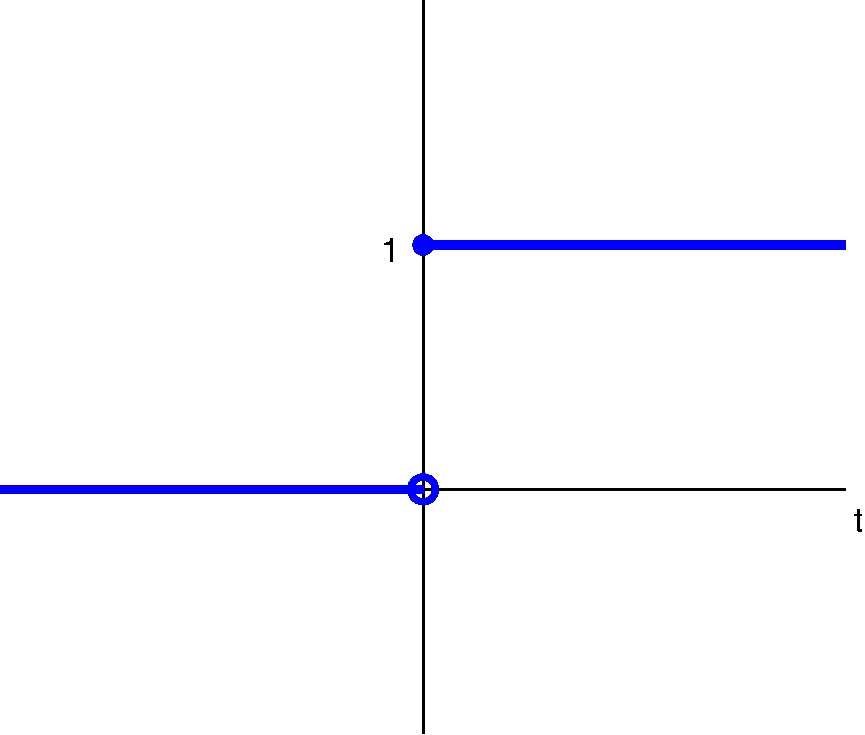
\includegraphics[width=\textwidth]{figs/unitstep}

\vspace{4mm}
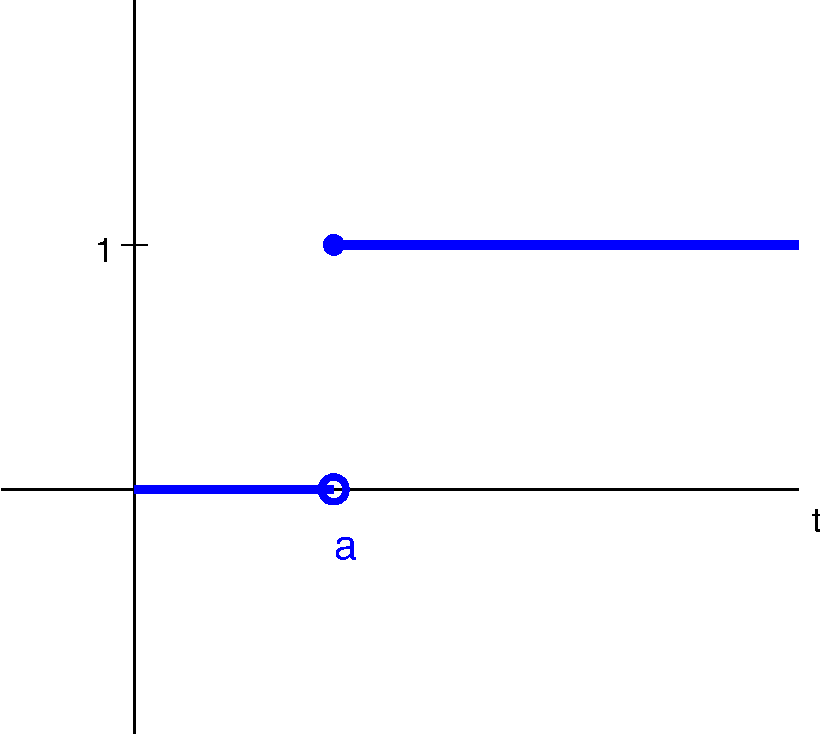
\includegraphics[width=\textwidth]{figs/unitsteptrans}
\end{column}
\end{columns}
\end{frame}


\begin{frame}{$\UU(t-a)$ helps with switching on/off}

\small
write each function in terms of unit step function(s):
\begin{itemize}
\item \emph{example A.} % 7.3 #57

\vspace{-3mm}
    $$f(t) = \begin{cases} 0, & 0 \le t < 1 \\ t^2, & t\ge 1 \end{cases} \hspace{70mm}$$

\vspace{6mm}
\item \emph{example B.} % 7.3 #74

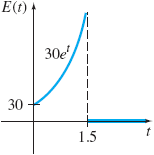
\includegraphics[width=25mm]{figs/Egoesoff}

\vspace{6mm}
\end{itemize}
\end{frame}


\begin{frame}{Laplace transform with $\UU(t-a)$}

\begin{columns}
\begin{column}{0.8\textwidth}
\begin{itemize}
\item $\UU(t)$ is also called the \emph{Heaviside} function
\item easy-to-show: if $F(s)=\LL{f(t)}$ then
    $$\LL{f(t-a)\UU(t-a)} = e^{-at} F(s)$$

\item \emph{show it:}

\vspace{40mm}
\end{itemize}
\end{column}
\begin{column}{0.2\textwidth}
\vspace{3mm}

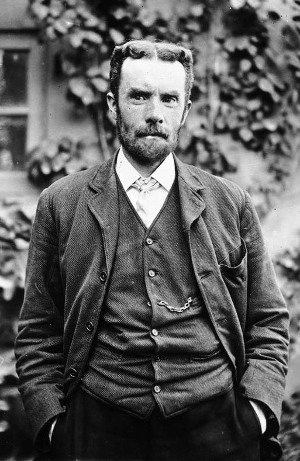
\includegraphics[width=0.7\textwidth]{figs/Heaviside}

\tiny
Oliver Heaviside

(1850--1925)

\vspace{5mm}
\hspace{-5mm} 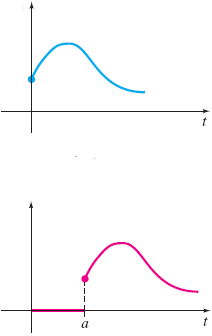
\includegraphics[width=1.2\textwidth]{figs/fanditstrans}
\end{column}
\end{columns}
\end{frame}


\begin{frame}{\#57 in \S7.3}

\begin{itemize}
\item \emph{exercise 5.}  write the function in terms of $\UU$ and then find the Laplace transform:

\vspace{-3mm}
    $$f(t) = \begin{cases} 0, & 0 \le t < 1 \\ t^2, & t\ge 1 \end{cases} \hspace{70mm}$$

\vspace{55mm}
\end{itemize}
\end{frame}


\begin{frame}{second version}

\begin{itemize}
\item the book then says:

\small
\begin{quote}
We are frequently confronted with the problem of finding the Laplace transform of a product of a function $g$ and a unit step function $\UU(t-a)$ where the function $g$ lacks the precise shifted form $f(t-a)$ in Theorem 7.3.2.
\end{quote}
\normalsize
\item yup, that's our problem
\item 2nd form of the same rule:
    $$\LL{g(t)\UU(t-a)} = e^{-at} \LL{g(t+a)}$$
\item it will be in the table also, when it is printed on quizzes/exams
\end{itemize}
\end{frame}


\begin{frame}{once again}

\begin{itemize}
\item \emph{exercise 5.}  write the function in terms of $\UU$ and then find the Laplace transform:

\vspace{-3mm}
    $$f(t) = \begin{cases} 0, & 0 \le t < 1 \\ t^2, & t\ge 1 \end{cases} \hspace{70mm}$$

\vspace{55mm}
\end{itemize}
\end{frame}


\begin{frame}{like \#66 in \S7.3}

\begin{itemize}
\item \emph{exercise 6.}  use Laplace transforms to solve the ODE IVP:
    $$y''+9y=f(t), \quad y(0)=0, \, y'(0)=0$$
where \,\, $\displaystyle f(t) = \begin{cases} 1, & 0 \le t < 1 \\ 0, & t\ge 1 \end{cases}$

\vspace{55mm}
\end{itemize}
\end{frame}


\begin{frame}{summary}

\begin{itemize}
\item assume $\LL{f(t)}=F(s)$
\item \emph{1st translation theorem}.
    $$\boxed{\LL{e^{at} f(t)} = F(s-a)}$$
\item \emph{2nd translation theorem}.  if $a>0$ then
    $$\boxed{\LL{f(t-a) \mathcal{U}(t-a)} = e^{-as} F(s)}$$

\vspace{-2mm}
    \begin{itemize}
    \item includes easy case: \, $\LL{\mathcal{U}(t-a)} = \frac{e^{-as}}{s}$
    \item second form
        $$\boxed{\LL{g(t) \mathcal{U}(t-a)} = e^{-as} \LL{g(t+a)}}$$
    \end{itemize}

\medskip
\item these are all in the table you will get on quizzes and exams, so:

\centerline{\alert{goal is understanding not memorizing}}
\end{itemize}
\end{frame}


\begin{frame}{expectations}

\begin{itemize}
\item just watching this video is \emph{not} enough!
     \begin{itemize}
     \item see ``found online'' videos and stuff at

     \centerline{\href{https://bueler.github.io/math302/week12.html}{\tt \color{cyan} bueler.github.io/math302/week12.html}}
     \item \emph{read} sections 7.3 and 7.4 in the textbook
         \begin{itemize}
         \item you can ignore ``beams'' and example 10 in \S7.3
         \item only 7.4.2 Transforms of Integrals in \S7.4
         \end{itemize}
     \item \emph{do} the WebAssign exercises for section 7.3
         \begin{itemize}
         \item I will quiz on problems like these
         \end{itemize}
     \end{itemize}
\end{itemize}
\end{frame}

\end{document}

